\chapter{Evaluation}


%In this chapter you should describe the previous (if possible) and final experiments performed on the implementation.

%Every single experiment should be explained individually, providing to the reader information about the meaning of the experiment, the expected (theoretical) results, the final results, the comparison between them and others (if possible) and the conclusions. 

%Each experiment should include a description, covering (when possible) the following information:
%\begin{itemize}
%	\item Significant physical features (obstacles present on the environment, human presence, temperature, humidity, possible noise sources, computational speed of the machine, etc.)
%	\item The precise location of the experiment (latitude and longitude, room number or citation to a description of the used laboratory).
%	\item Sampling design (variable(s) measured, transformation performed to the data, samples collected, replication, comparative with a Ground Truth system, collecting data protocol).
%	\item Analysis design (how the data are processed, statistical procedures used, statistical level to determine significance).
%\end{itemize}
%The provided information should be sufficient to allow other scientists to repeat your experiment in the same conditions. Thus, the use of standard and well-known equipment could only be represented by a simple sentence, but the non-standard equipment should be described in detail, citing the source (vendor) and most important characteristics.

%To write it, try to use the third person when describing the experiments and results. Avoid to use first person. Past tense should be the dominant conjugation (the work is done and was performed in the past).

%Note: Graphics represent really well data, use them! (Matlab or Octave could be useful for that).



In the system, cost functions are importent because an accurate cost function can improve the efficiency of task allocation. Followings are goals of experiments:

\begin{itemize}
	\item Evaluate the need of decision variables.
	\item Find the best weight combinations in cost functions.
	\item Evaluate the hypothesis that the more robots, the faster to complete a task set, the higher the completion rate.
%	\item Investigate how different weight combinations in cost functions affact the performance \cite{Shiqi}. 
\end{itemize}

\section{Experiment Setup}

\begin{enumerate}
    \item Run Gazebo and load office world model (Figure \ref{fig:gazebo_model}). 
    \item Configure word property. For example, the simulation time were configured as ``2020-06-01 9:00:00''.
    \item Use SLAM \cite{slam} to create a map for the office model(Figure \ref{fig:exp_map}).
    \item Start SQL server and Charging event in database \ref{fig:charging_station_event}.
    \item Start ROS nodes including ``centralized pool'', ``robot controller'', ``sensor simulatior'' and ``charging station''.
\end{enumerate}

\begin{figure}[htbp]
	\centering
	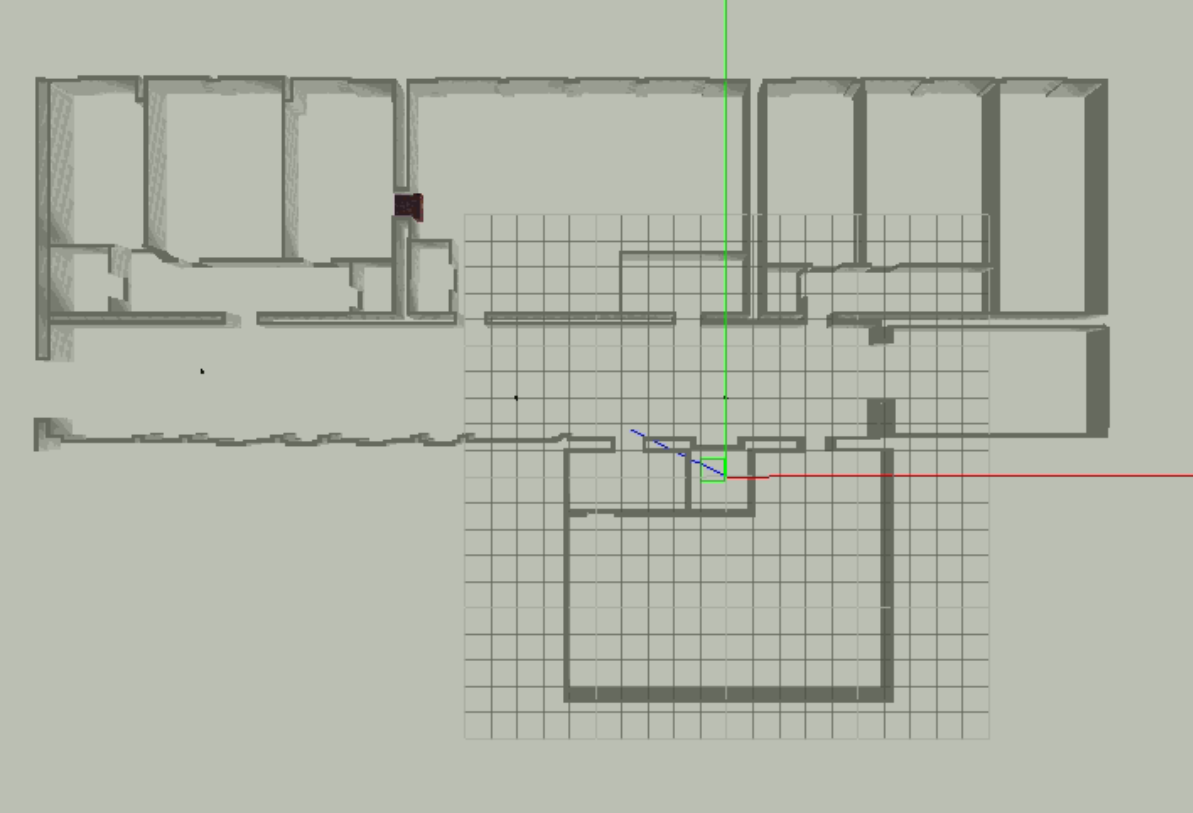
\includegraphics[width = 0.7\textwidth]{content/images/ch5/gazebo_model.png}
	\caption{Gazebo Simulation}
	\label{fig:gazebo_model}
\end{figure}

\begin{figure}[htbp]
    \centering
    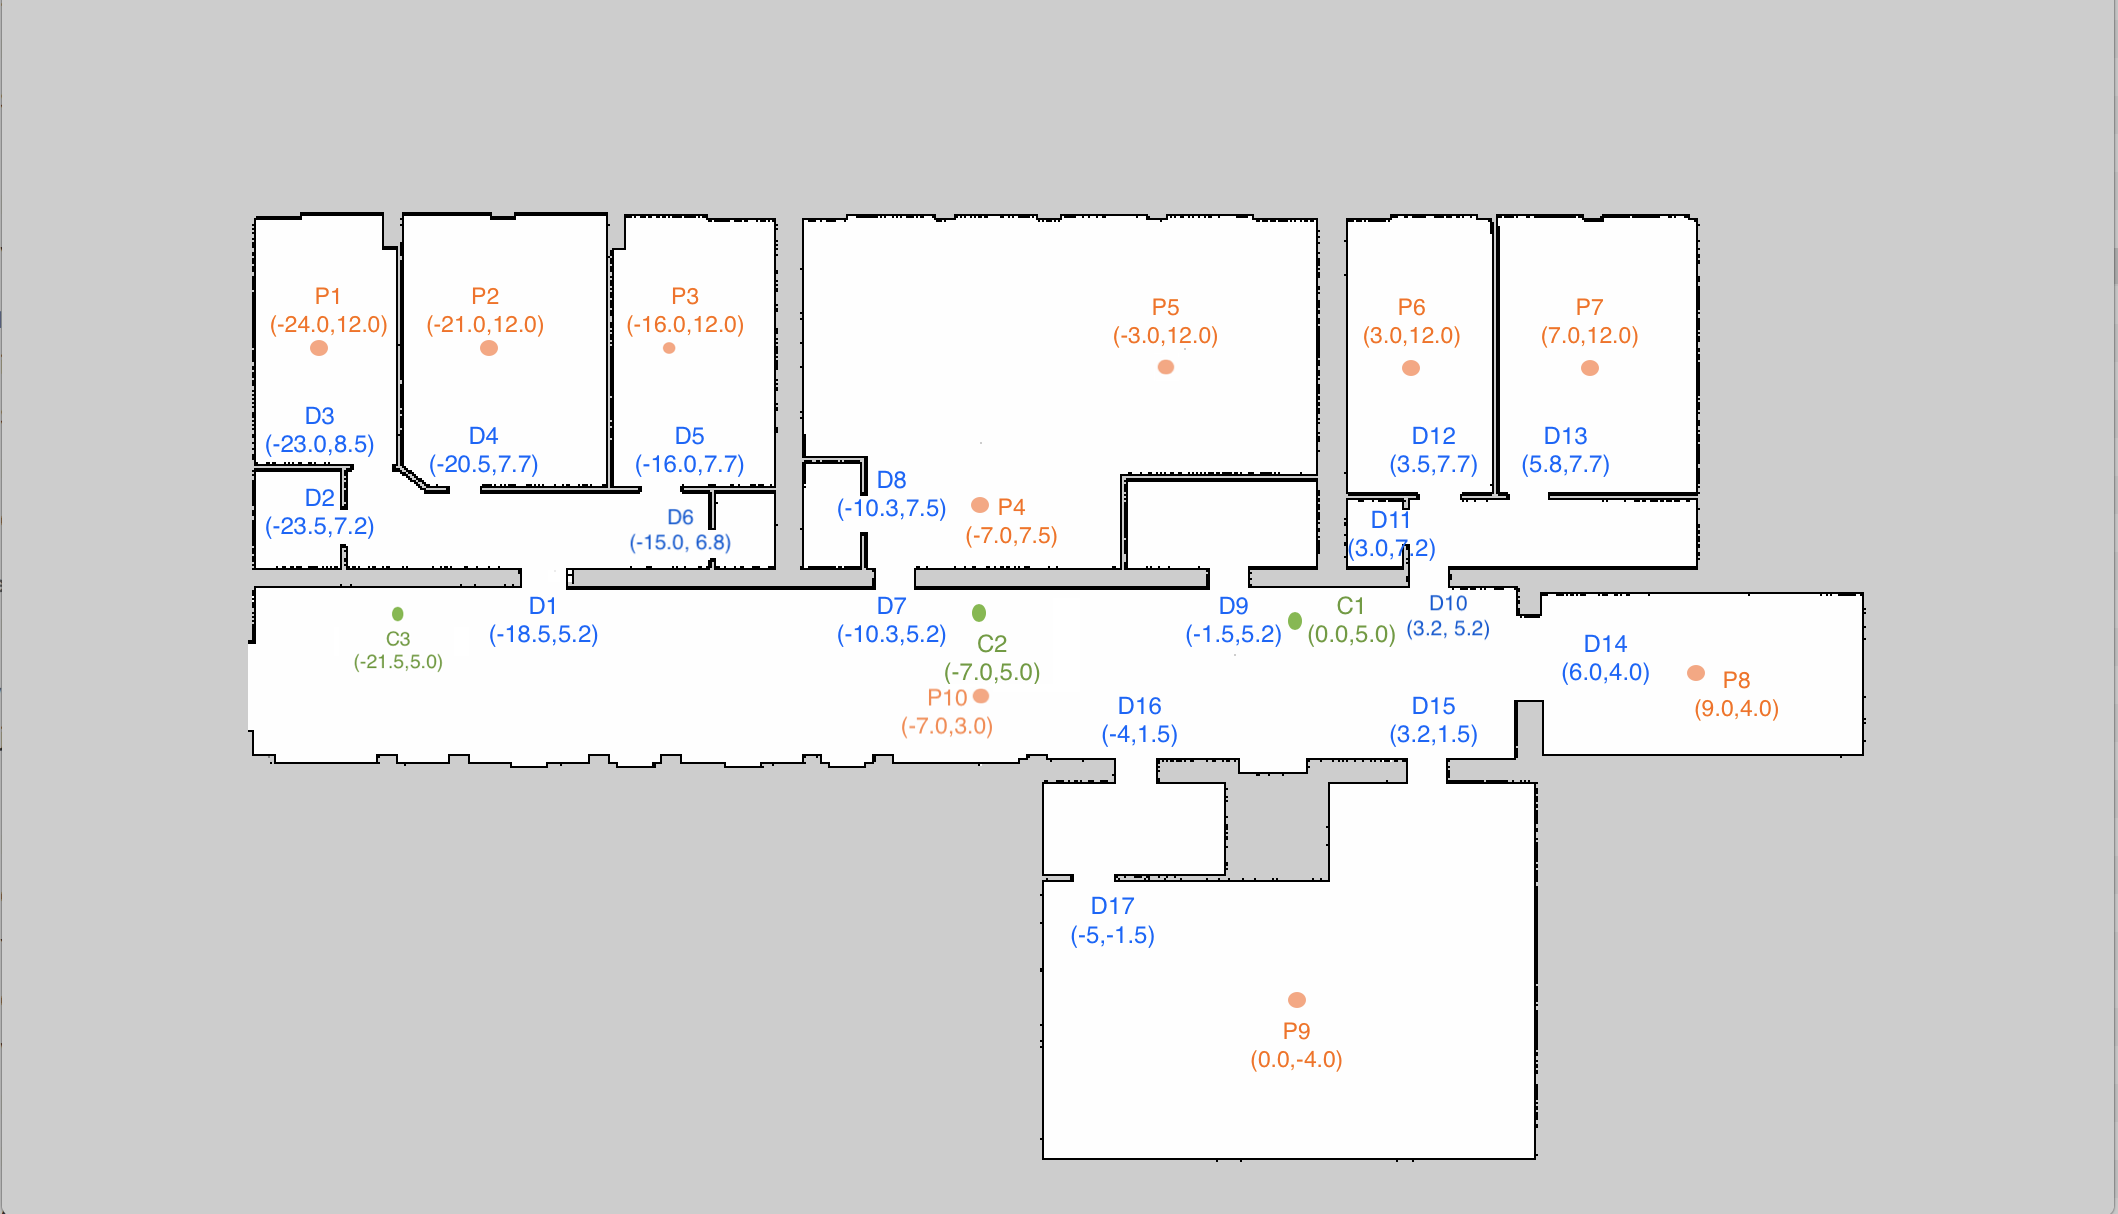
\includegraphics[width = 0.9\textwidth]{content/images/ch5/door_station_points.png}
    \caption{Experiment Map}
    \label{fig:exp_map}
\end{figure}



\section{Sensor Simulator}
\label{sec:sensor_simulatior}

\paragraph{Sensor Message Publish}
In this project, a sensor simulator node is used to publish measurement results. The door simulator publish one messages for each door periodically to a ROS topic ``sensor data''. The message contains door id, sensor position and door status(Table \ref{sec:measurement_message}). The door status are created according to open possibilities table (Table \ref{tab:db_open_possibilities}). 


\paragraph{Door Status Generation}
For example, on monday (day of week is 2) at simulation time ``10:30:00'' (on timeslot 10:00:00-10:59:59), in 80\% possibility a ``door open'' is generated and in 20\% a ``door closed'' is generated (Initialized Open Possibility is 0.80).


\paragraph{Sensor Message Subscribe}
The process of sensor simulation is shown in Figure \ref{sec:sensor_simulatior}. The robots (robot controller nodes) subscribe the same ROS topic ``sensor data''. Every time the sensor simulator sends a message, all robots will receive this message at the same time. Their distance filters filter sensor messages with position outside the comminication range and keep sensor messages within the communication range. With this process, the sensor simulatior sends instant measurement result to robots within communication range. However, if the system is applied to the real world, instead of sending instant measurement result, the real world sensor could send a record with history measurement.

\begin{figure}
\centering
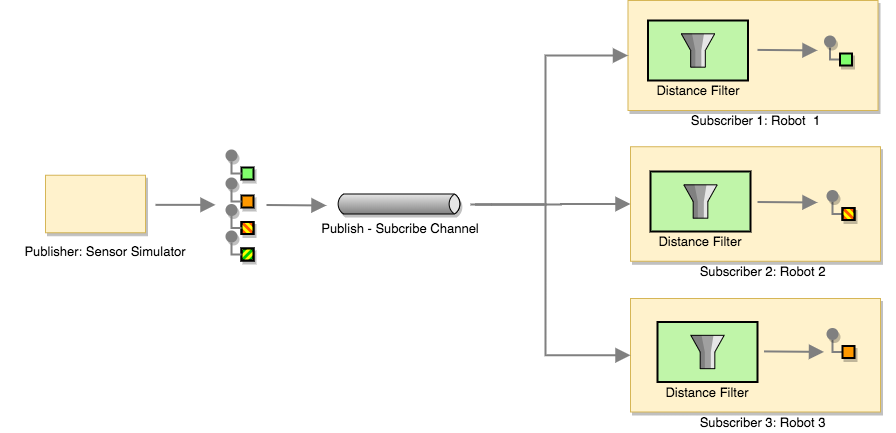
\includegraphics[width = 0.7\textwidth]{content/images/ch4/sensor_simulator.drawio.png}
\caption{Sensor Simulator}
\label{fig:sensor_simulator}
\end{figure}

\section{Enviroment Task Evaluation Experiment}


\subsection{Experiment: Use Enumeration Method to Find the Best Weight Combinations}
\label{sec:enviroment_experiment_enumerate}
\paragraph{Experiment Introduction} To find the best weight combinations, 30 experiemnt are created with $W_{\mbox{battery consumption}} \in \{ 0,1,5,10 \},  W_{\mbox{update}} \in \{-10,-5,-1\}, W_{\mbox{possibility}} \in \{-10,-5,-1,0\}$. In addition, the conditions $W_{\mbox{update}}=0$ was not testable, because during the experiment centralized pool generate the same ``gather enviroment information tasks``, which let robots not moving and measuring their nearest door. Experiment Duration T = 10 min.

\paragraph{Sampling Design} When simulation started, robots ran charging task (Task 1-3) at their charging station and started charging (Figure \ref{fig:charging_station_event}). For example, robot 1 charged at charging staion 1, robot 2 charged at charging staion 2, robot 3 charged at charging staion 3. When robot fully charged, the first experiment started (Figure \ref{tab:env_exp_timeline}). After that, the task allocation module in centralized pool created a ``gather enviroment information task'' to each robot requested a task. After a constant experiment duration T, experiments were finished and robots went to their charging stations. These rules ensured that 1) Each Robot always started at an initial position. 2) Robots would not shut down because of power exhaustion. 3) Robots spent the same time gathering enviroment information.

\begin{figure}[htbp]
    \centering
    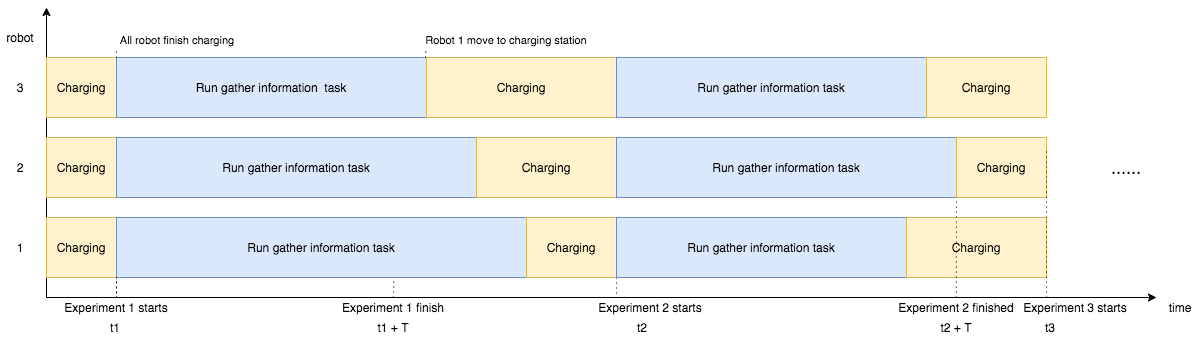
\includegraphics[width = 0.7\textwidth]{content/images/ch5/env_exp_timeline.drawio.png}
    \caption{Enviroment Task Experiment Timeline}
    \label{tab:env_exp_timeline}
\end{figure}

\paragraph{Analysis design} The experiment start time was when all robot finshed charging and started request task (Figure \ref{tab:env_exp_timeline}). The experiment duraion is a constant value T. The experiment finish time $T_{\mbox{finish time}} = T_{\mbox{start time}} + T $. Some important factors are evaluated. 

\begin{itemize}
    \item \textsl{Last update.} The ``last update'' factor is the time difference between experiment start time and minial value in ``last update'' column in door table (Table \ref{tab:db_doors}) when an experiment finished. For example, ``last update'' factor in experiment 1 (Figure \ref{fig:enviroment_experiment_enumerate})  is ``00:02:57''. It means that the door in the worst case not be measured since 2 minites 57 seconds after experiment start.
    \item \textsl{Average Update Interal} The ``Average update Interal'' means the average interval of door update. For example, ``Average Update Interal'' factor in experiment 1 (Figure \ref{fig:enviroment_experiment_enumerate}) is ``00:01:00''. It means that on average, every door is updated every minute.
    \item \textsl{Succedded task.} The ``Number of task'' factor  means the number of succeeded ``gather enviroment information'' task.
\end{itemize}

\paragraph{Experiemnt Result} 
Figure \ref{fig:enviroment_experiment_enumerate} represent the experiemnt result.

\paragraph{Expariment Analysis} 

As shown in experiment result, all ``Minial Last Update'' value is from 1 min to 5 min, which is much less than experiment duraion (10 min). It means some doors were not timely updated information. One possible reason is that the velocity of robot is small (about 0.2 per second), the experiemnt duraion (10min) was not long enough to let three robot pass to all doors. Another possible reason is that the robot's route is partially duplicated. For example, when system started, robot 1 was in charging station 1 and got a task to door 3, while robot 2 was in charging station 2 and got a task to door 4. As shown in Figure \ref{fig:positions_door_station}, these two route are partially duplicated, both of them pass through door 1 and entered room 1 (Figure \ref{fig:room_division}). The idealy solution was to give both task to one robot. 

\begin{figure}[htbp]
    \centering
    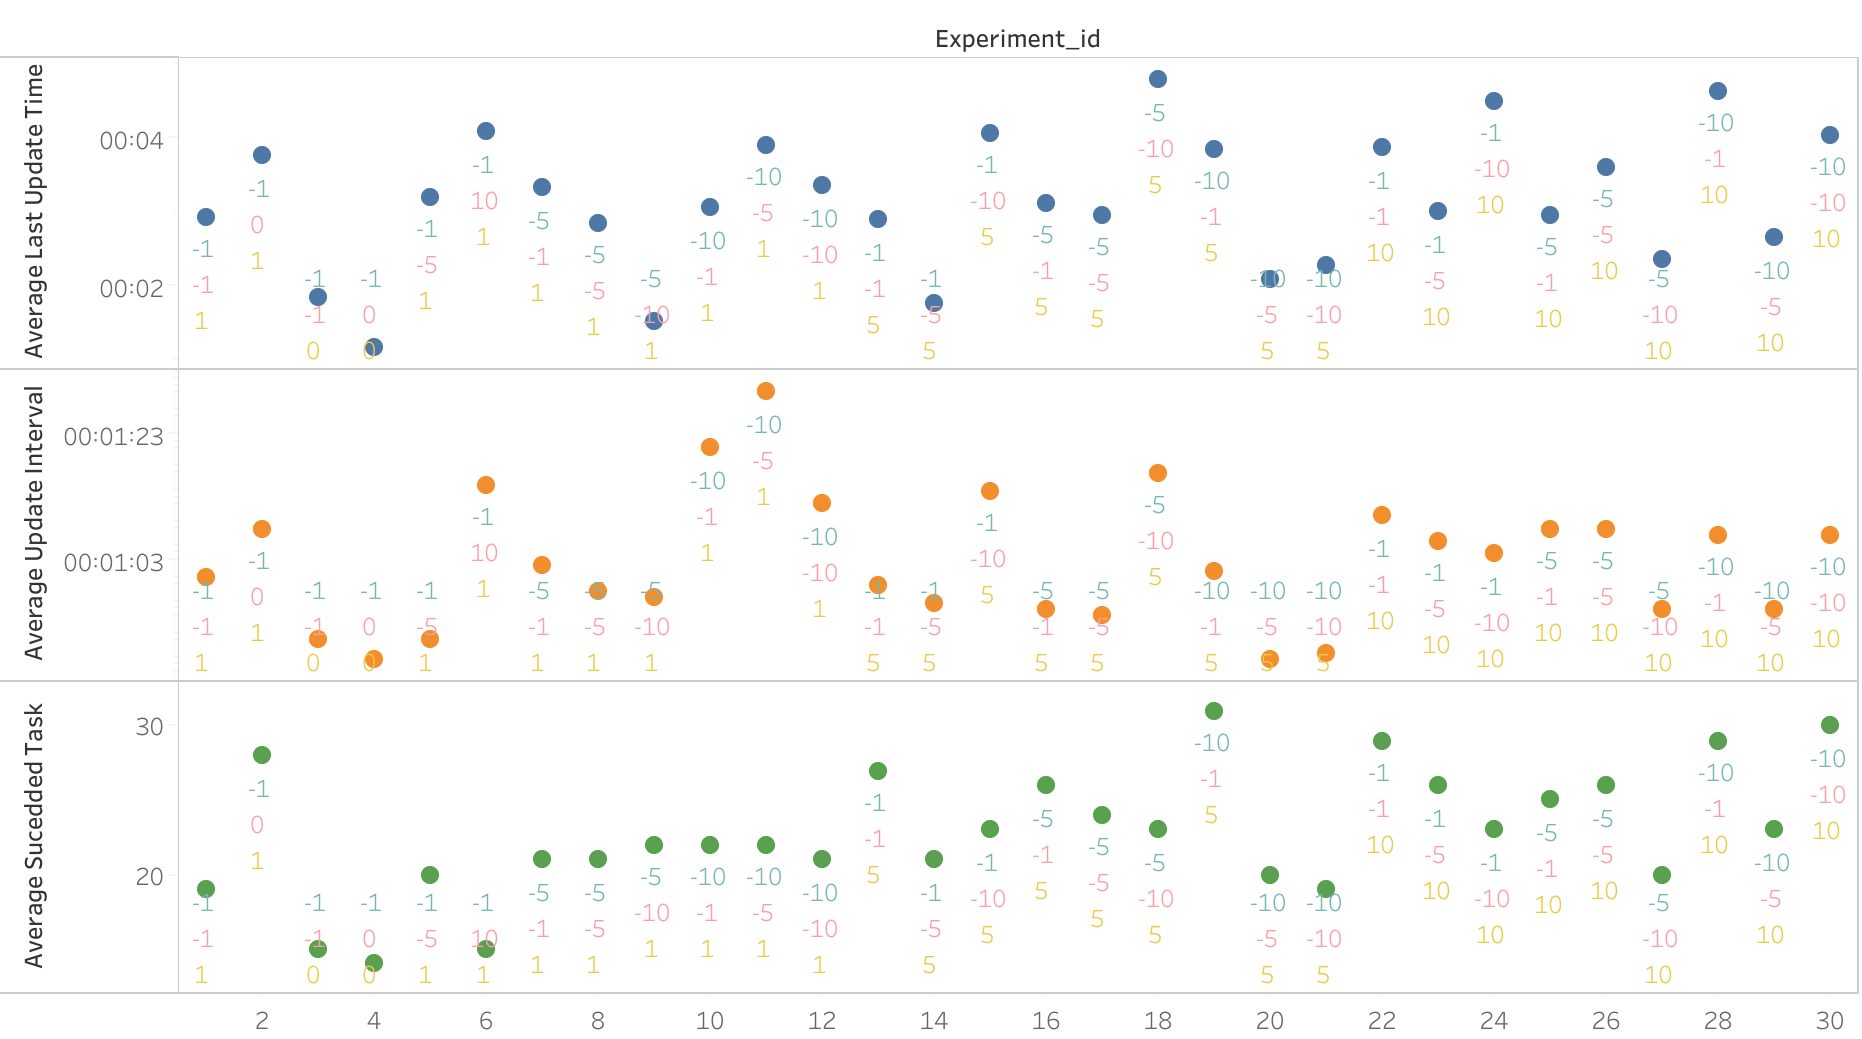
\includegraphics[width = 0.9\textwidth]{content/images/ch5/enviroment_enumerate.png}
    \caption{Experiment: Use enumeration method to find best weight combination}
    \text{Green: $W_{\mbox{battery}}$ Pink: $ W_{\mbox{possibility}}$ Yellow: $W_{\mbox{update}} $}
    \label{fig:enviroment_experiment_enumerate}
\end{figure}


\subsection{Experiment: Use Analysis to Find the Best Weight Combinations}

\paragraph{Experiment Introduction} 
As is discussed in last experiemnt (Section \ref{sec:enviroment_experiment_enumerate}), the experiment time was too short to allow the robot to explore each door. Therefore, the experiemnt duraion in this experiemnt was increased to 20 min.
Firstly, we shuold find the best weight combination $W_{\mbox{battery}}$ and $ W_{\mbox{update}}$, then find the third weight value $W_{\mbox{possibility}}$. Finally, the best combination of weight will be concluded.
 According to cost table (Figure \ref{fig:cost_table}), the update time value has a minial value of 6.986 and a maximal value of 336.986 (column 3), which are much larger than battery comsumption (column 2) and product of door open possibilities (column 4).
  Therefore, 18 experiments are created with $W_{\mbox{battery}}$
   = 0.1  and $W_{\mbox{battery}} \in \{1,5,10,15,20,25 \}$.

\paragraph{Sampling Design} When simulation started, robots ran charging task (Task 1-3) at their charging station and started charging (Figure \ref{fig:charging_station_event}). For example, robot 1 charged at charging staion 1, robot 2 charged at charging staion 2, robot 3 charged at charging staion 3. When robot fully charged, the first experiment started (Figure \ref{tab:env_exp_timeline}). After that, the task allocation module in centralized pool created a ``gather enviroment information task'' to each robot requested a task. After a constant experiment duration T, experiments were finished and robots went to their charging stations. These rules ensured that 1) Each Robot always started at an initial position. 2) Robots would not shut down because of power exhaustion. 3) Robots spent the same time gathering enviroment information.

\paragraph{Analysis design} The experiment start time was when all robot finshed charging and started request task (Figure \ref{tab:env_exp_timeline}). The experiment duraion is a constant value T. The experiment finish time $T_{\mbox{finish time}} = T_{\mbox{start time}} + T $. Some important factors are evaluated. 
\begin{itemize}
    \item \textsl{Last update.} The ``last update'' factor is the time difference between experiment start time and minial value in ``last update'' column in door table (Table \ref{tab:db_doors}) when an experiment finished. For example, ``last update'' factor in experiment 1 (Figure \ref{fig:enviroment_experiment_enumerate}) is ``00:02:57''. It means that the door in the worst case not be measured since 2 minites 57 seconds after experiment start.
    \item \textsl{Average Update Interal} The ``Average update Interal'' means the average interval of door update. For example, ``Average Update interal'' factor in experiment 1 is ``00:01:00''. It means that on average, every door is updated every 1 minute.
    \item \textsl{Succedded task.} The ``Number of task'' factor  means the number of succeeded ``gather enviroment information'' task.
\end{itemize}

\begin{figure}[htbp]
    \centering
    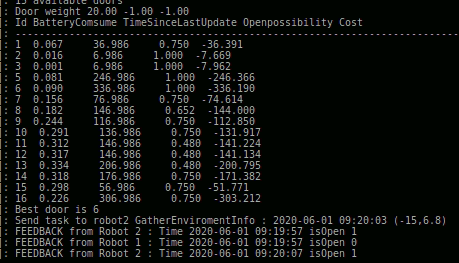
\includegraphics[width = 0.7\textwidth]{content/images/ch5/weight_analyze.png}
    \caption{Centralized Pool Cost Table}
    \label{fig:cost_table}
\end{figure}

\paragraph{Expariment Result} The experiemnt results are shown in Figure \ref{fig:enviroment_experiment_two_value} and Figure \ref{fig:enviroment_experiment_three_value}
\begin{figure}[htbp]
    \centering
    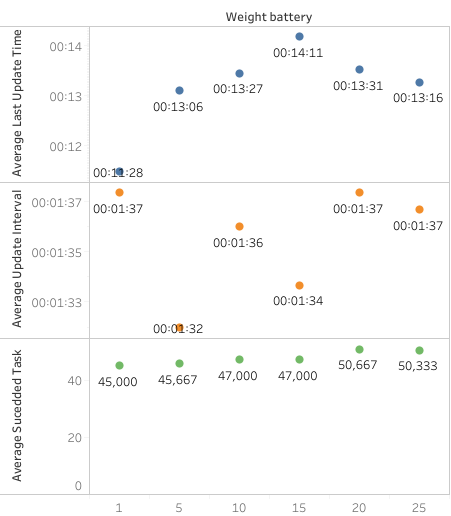
\includegraphics[width = 0.7\textwidth]{content/images/ch5/enviroment_change_weight_battery_only.png}
    \caption{Experiment: Change $W_{\mbox{battery}}$ under condition $W_{\mbox{update}} = 0.1$ and $W_{\mbox{possibility}}=0$}
    \label{fig:enviroment_experiment_two_value}
\end{figure}


\begin{figure}[htbp]
    \centering
    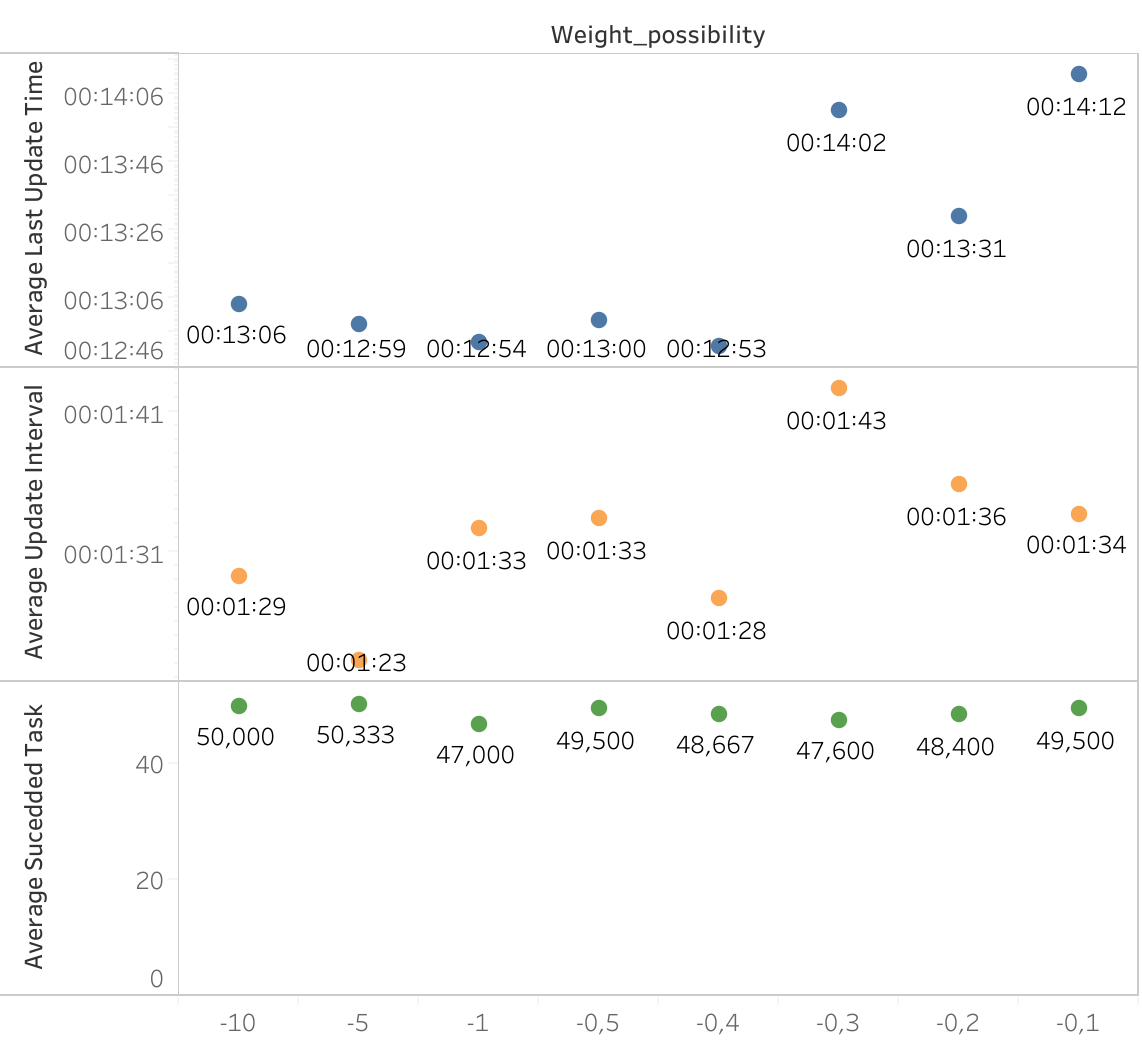
\includegraphics[width = 0.7\textwidth]{content/images/ch5/enviroment_change_weight_possibility_only.png}
    \caption{Experiment: Change $W_{\mbox{possibility}}$ under condition $W_{\mbox{battery}}=15$ and $ W_{\mbox{update}}=0.1$}
    \label{fig:enviroment_experiment_three_value}
\end{figure}

\paragraph{Expariment Analysis} 
As shown in experiemnt result Figure \ref{fig:enviroment_experiment_two_value}, ``weight battery'' increased from 0 to 25, the ``average succedded experiment task number'' slighly increased from 45 to 50, but ``average update interval'' were floated in a small range around ``00:01:35''. Especially, as ``weight battery'' increased from 0 to 15, ``average last update'' showed an upward trend, and as ``weight battery'' increased from 15 to 25, ``average last update'' showed a downward trend, 
therefore ``weight battery'' 15 and ``weight update'' 0.1 was the best combination. 
This combination was used in next experiemnt set (Figure \ref{fig:enviroment_experiment_three_value}). From this experiemnt set, it was concluded that ``weight battery'' 15, ``weight update'' 0.1, ``weight possibility'' 0.1 and ``weight battery'' 15, ``weight update'' 0.1, ``weight possibility'' -0.3 were two best weight combinations for enviroment cost function.

\section{Execute Task Evaluation Experiment}

\subsection{Experiment: Impact of Decision Variables}

\paragraph{Experiment Introduction} 
This set of experiments evaluated the need of four decision variables: battery consumption, waiting time, product of door open possibility and priority. 

\paragraph{Sampling design}
Table \ref{tab:db_task_table} shows "task table" in database. At this point, robots finished task 4-21 in experiment 1 and finished 21-39 in experiment 2. When simulation started, 3 robots ran charging task (Task 1-3) and moved to corresponding charging station and started charging (Figure \ref{fig:charging_station_event}). For example, robot 1 charged at charging staion 1, robot 2 charged at charging staion 2, robot 3 charged at charging staion 3. 
When robot fully charged, the first experiment started (Figure \ref{fig:execute_task_experiment_timeline}), and 15 ``execute tasks'' and 3 ``charging tasks'' were created (Task 4-21). Especially, in the same experiment, the task interal were the same (Table \ref{tab:db_task_table}). In different experiment, the corresponding task had the same goal positions (Task 4 and 21, Task 4 and 22). 
When all robot finished tasks, the experiment would be finished and robots charged at previous charging station(Task 19-21).
These rules ensured that robot not only started at their initial positions but also processed same task set and not shuted down because of power exhaustion.


\begin{figure}[htbp]
    \centering
    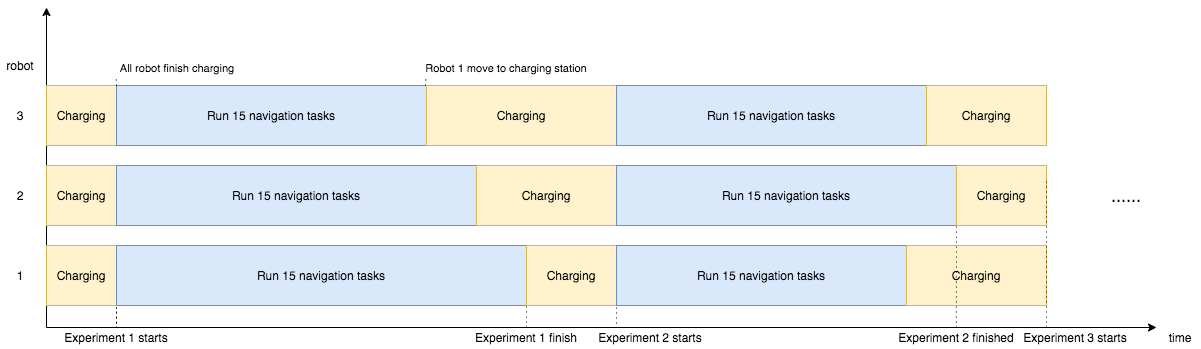
\includegraphics[width = 0.9\textwidth]{content/images/ch5/exe_exp_timeline.drawio.png}
    \caption{Execute Task Experiment Timeline}
    \label{fig:execute_task_experiment_timeline}
\end{figure}


\begin{table}[]
\resizebox{\textwidth}{!}{
\begin{tabular}{|c|c|c|c|c|c|c|c|c|c|}
\hline
Task ID & Task Name & Start Time    & Target ID & Robot ID &Priority & Task Status & Dependency & Finish Time & Description \\ \hline
1 & Charging    & NULL                & 18 & 1 & 5 & Succedded & 0 & 2020-06-02 11:03:12 & Succeeded \\ \hline
2 & Charging    & NULL                & 19 & 2 & 5 & Succedded & 0 & 2020-06-02 11:03:12 & Succeeded \\ \hline
3 & Charging    & NULL                & 20 & 3 & 5 & Succedded & 0 & 2020-06-02 11:03:11 & Succeeded \\ \hline
4 & ExecuteTask & 2020-06-02 11:04:17 & 21 & 3 & 2 & Succedded & 0    & 2020-06-02 11:05:16 & Succeeded \\ \hline
5 & ExecuteTask & 2020-06-02 11:05:22 & 22 & 1 & 2 & Succedded & 0    & 2020-06-02 11:07:29 & Succeeded \\ \hline
6 & ExecuteTask & 2020-06-02 11:06:27 & 23 & 2 & 2 & Succedded & 0    & 2020-06-02 11:08:06 & Succeeded \\ \hline
7 & ExecuteTask & 2020-06-02 11:07:32 & 24 & 3 & 2 & Succedded & 0    & 2020-06-02 11:09:25 & Succeeded \\ \hline
8 & ExecuteTask & 2020-06-02 11:08:37 & 25 & 1 & 2 & Succedded & 0    & 2020-06-02 11:10:46 & Succeeded \\ \hline
9 & ExecuteTask & 2020-06-02 11:09:42 & 26 & 2 & 2 & Succedded & 0    & 2020-06-02 11:12:42 & Succeeded \\ \hline
10 & ExecuteTask & 2020-06-02 11:10:47 & 27 & 3 & 2 & Succedded & 0    & 2020-06-02 11:12:56 & Succeeded \\ \hline
11 & ExecuteTask & 2020-06-02 11:11:52 & 28 & 1 & 2 & Succedded & 0    & 2020-06-02 11:14:13 & Succeeded \\ \hline
12 & ExecuteTask & 2020-06-02 11:12:57 & 29 & 2 & 2 & Succedded & 0    & 2020-06-02 11:14:20 & Succeeded \\ \hline
13 & ExecuteTask & 2020-06-02 11:14:02 & 30 & 3 & 2 & Succedded & 0    & 2020-06-02 11:15:36 & Succeeded \\ \hline
14 & ExecuteTask & 2020-06-02 11:15:07 & 21 & 1 & 2 & Succedded & 0    & 2020-06-02 11:18:07 & Succeeded \\ \hline
15 & ExecuteTask & 2020-06-02 11:16:12 & 22 & 2 & 2 & Succedded & 0    & 2020-06-02 11:18:49 & Succeeded \\ \hline
16 & ExecuteTask & 2020-06-02 11:17:17 & 23 & 3 & 2 & Succedded & 0    & 2020-06-02 11:18:58 & Succeeded \\ \hline
17 & ExecuteTask & 2020-06-02 11:18:22 & 24 & 1 & 2 & Succedded & 0    & 2020-06-02 11:20:14 & Succeeded \\ \hline
18 & ExecuteTask & 2020-06-02 11:19:27 & 25 & 2 & 2 & Succedded & 0    & 2020-06-02 11:21:36 & Succeeded \\ \hline
19 & Charging    & NULL                & 18 & 1 & 5 & Succedded & 0 & 2020-06-02 11:23:08 & Succeeded \\ \hline
20 & Charging    & NULL                & 19 & 2 & 5 & Succedded & 0 & 2020-06-02 11:23:08 & Succeeded \\ \hline
21 & Charging    & NULL                & 20 & 3 & 5 & Succedded & 0 & 2020-06-02 11:23:08 & Succeeded \\ \hline
22 & ExecuteTask & 2020-06-02 11:24:13 & 21 & 3 & 2 & Succedded & 0 & 2020-06-02 11:25:12 & Succeeded \\ \hline
23 & ExecuteTask & 2020-06-02 11:25:18 & 22 & 2 & 2 & Succedded & 0 & 2020-06-02 11:26:54 & Succeeded \\ \hline
24 & ExecuteTask & 2020-06-02 11:26:23 & 23 & 1 & 2 & Succedded & 0 & 2020-06-02 11:28:35 & Succeeded \\ \hline
25 & ExecuteTask & 2020-06-02 11:27:28 & 24 & 3 & 2 & Succedded & 0 & 2020-06-02 11:29:23 & Succeeded \\ \hline
26 & ExecuteTask & 2020-06-02 11:28:33 & 25 & 2 & 2 & Succedded & 0    & 2020-06-02 11:30:41 & Succeeded \\ \hline
27 & ExecuteTask & 2020-06-02 11:29:38 & 26 & 1 & 2 & Succedded & 0    & 2020-06-02 11:32:37 & Succeeded \\ \hline
28 & ExecuteTask & 2020-06-02 11:30:43 & 27 & 3 & 2 & Succedded & 0    & 2020-06-02 11:32:54 & Succeeded \\ \hline
29 & ExecuteTask & 2020-06-02 11:31:48 & 28 & 2 & 2 & Succedded & 0    & 2020-06-02 11:34:09 & Succeeded \\ \hline
30 & ExecuteTask & 2020-06-02 11:32:53 & 29 & 1 & 2 & Succedded & 0    & 2020-06-02 11:34:15 & Succeeded \\ \hline
31 & ExecuteTask & 2020-06-02 11:33:58 & 30 & 3 & 2 & Succedded & 0    & 2020-06-02 11:35:32 & Succeeded \\ \hline
32 & ExecuteTask & 2020-06-02 11:35:03 & 21 & 2 & 2 & Succedded & 0    & 2020-06-02 11:38:03 & Succeeded \\ \hline
33 & ExecuteTask & 2020-06-02 11:36:08 & 22 & 1 & 2 & Succedded & 0    & 2020-06-02 11:38:45 & Succeeded \\ \hline
34 & ExecuteTask & 2020-06-02 11:37:13 & 23 & 3 & 2 & Succedded & 0    & 2020-06-02 11:38:54 & Succeeded \\ \hline
35 & ExecuteTask & 2020-06-02 11:38:18 & 24 & 2 & 2 & Succedded & 0    & 2020-06-02 11:40:11 & Succeeded \\ \hline
36 & ExecuteTask & 2020-06-02 11:39:23 & 25 & 1 & 2 & Succedded & 0    & 2020-06-02 11:41:40 & Succeeded \\ \hline
37 & Charging    & NULL                & 18 & 1 & 5 & Succedded & 0 & 2020-06-02 11:43:45 & Succeeded \\ \hline
38 & Charging    & NULL                & 19 & 2 & 5 & Succedded & 0 & 2020-06-02 11:43:45 & Succeeded \\ \hline
39 & Charging    & NULL                & 20 & 3 & 5 & Succedded & 0 & 2020-06-02 11:43:45 & Succeeded \\ \hline
\end{tabular}}
\caption{Task Table}
\label{tab:exp_task_table}
\end{table}

\paragraph{Analysis design}
As is discussed in last paragraph, in each experiemnts, robots need to finish 15 ``execute tasks'' and 3 ``charging tasks''.
The experiment start time was when all robot finshed charging and started request task (Figure \ref{fig:execute_task_experiment_timeline}), and the experiment finish time was when the latest task is finished.
The experiment duration was an important evaluation factor, which was the time difference between experiment start time and experiment finished time.  
There end state of ``execute tasks'' were evaluated. In an experiment result table, the ``Succeeded'' column counted the tasks ended with ``Succeeded'' state, the ``Expired'' column counted the tasks ended with ``Succeeded'' state, the ``Failed'' column counted the tasks ended with ``Runing'', ``Error'', ``Canceled'', ``To rerun'' states. 
Table \ref{tab:exp_decision_variables} is an example of experiment result. 

\paragraph{Experiment Result} 
The experiment result (Table \ref{tab:exp_decision_variables}.) shows that in experiment 1, all 15 task were succesfully finsihed with minimalexperiment duraion. In experiment 2, 4, 5 mores than half of the task were expired. In experiment 3, all tasks were successfully finished but it took more time than experiment 1. 
The experiment 6-24 (Table \ref{tab:only_one_desition_variable_changed} and Figure \ref{tab:only_one_desition_variable_changed}) evaluated each decision variable sepratelly. 
\paragraph{Experiment Analysis.} 
Comparing experiment 1-5, it was concluded that the cost function with multiple decision variables had better performance than a cost function with single decition variable. However, according to experiment 6-24, the ``experiment duration'' changed very little when only one desition variable changed others unchanged, therefore how each decision variable affect the task allocation is still unknown.

\begin{table}[htb]
\centering
\resizebox{\textwidth}{!}{
\begin{tabular}{|c|c|c|c|c|c|c|c|c|c|c|c|} 
\hline
Experiment & $W_{\mbox{battery}}$ & $W_{\mbox{waiting time}}$ & $W_{\mbox{door open possibility}}$	&  $W_{\mbox{priority}}$ & Experiment Duration &Total Task & Succedded Task &	Expired Task & Failed Task	 \\
\hline
1	& 1.00 &	 1.00 &	 -1.00&  -1.00&	 00:18:23 &	 15 &	 15 &	 0 & 0	 \\\hline
2	& 1.00 &	 0.00 &	 0.00 &	 0.00 &	 00:17:23 &	 15 &	 7 &	 8 & 0	\\ \hline
3	& 0.00 &	 1.00 &	 0.00 &	 0.00 &	 00:18:56 &	 15 &	 15 &	 0 & 0	 \\\hline
4	& 0.00 &	 0.00 &	 -1.00 & 0.00 &	 00:18:41 &	 15 &	 5 &	 10 & 0	\\\hline	 
5	& 0.00 &	 0.00 &	 0.00 &	 -1.00&	 00:17:21 &	 15 &	  3 &	 12 & 0	 \\	 \hline
\end{tabular}}
\caption{Runing execute task with single decision variable and multiple decision variables}
\label{tab:exp_decision_variables}
\end{table}

\begin{table}[]
\resizebox{\textwidth}{!}{
\begin{tabular}{|l|l|l|l|l|l|l|l|l|l|}
\hline
Experiment & $W_{\mbox{battery}}$ & $W_{\mbox{waiting time}}$ & $W_{\mbox{door open possibility}}$	&  $W_{\mbox{priority}}$ & Experiment Duration &Total Task & Succedded Task &	Expired Task & Failed Task	  \\ \hline
6       & 20      & 1        & -1      & -1      & 00:09:26 & 15    & 10        & 5       & 0        \\ \hline
7       & 40      & 1        & -1      & -1      & 00:09:48 & 15    & 10        & 5       & 0        \\ \hline
8       & 60      & 1        & -1      & -1      & 00:09:50 & 15    & 10        & 5       & 0        \\ \hline
9       & 80      & 1        & -1      & -1      & 00:09:47 & 15    & 10        & 5       & 0        \\ \hline
10       & 100     & 1        & -1      & -1      & 00:09:06 & 15    & 10        & 5       & 0        \\ \hline
11      & 1       & 20       & -1      & -1      & 00:09:48 & 15    & 10        & 5       & 0        \\ \hline
12       & 1       & 40       & -1      & -1      & 00:09:38 & 15    & 9         & 5       & 0        \\ \hline
13       & 1       & 60       & -1      & -1      & 00:10:09 & 15    & 10        & 5       & 0        \\ \hline
14       & 1       & 80       & -1      & -1      & 00:09:46 & 15    & 10        & 5       & 0        \\ \hline
15      & 1       & 100      & -1      & -1      & 00:10:01 & 15    & 10        & 5       & 0        \\ \hline
16      & 1       & 1        & -20     & -1      & 00:09:48 & 15    & 10        & 5       & 0        \\ \hline
17      & 1       & 1        & -40     & -1      & 00:09:50 & 15    & 10        & 5       & 0        \\ \hline
18      & 1       & 1        & -60     & -1      & 00:10:24 & 15    & 10        & 5       & 0        \\ \hline
19      & 1       & 1        & -80     & -1      & 00:09:48 & 15    & 10        & 5       & 0        \\ \hline
20      & 1       & 1        & -100    & -1      & 00:09:35 & 15    & 10        & 5       & 0        \\ \hline
21      & 1       & 1        & -1      & -20     & 00:10:22 & 15    & 10        & 5       & 0        \\ \hline
22      & 1       & 1        & -1      & -40     & 00:10:02 & 15    & 10        & 5       & 0        \\ \hline
23      & 1       & 1        & -1      & -60     & 00:09:48 & 15    & 10        & 5       & 0        \\ \hline
24      & 1       & 1        & -1      & -80     & 00:09:51 & 15    & 10        & 5       & 0        \\ \hline
\end{tabular}}
\caption{only one desition variable changed others unchanged}
\label{tab:only_one_desition_variable_changed}
\end{table}

\begin{figure}[htbp]
    \centering
    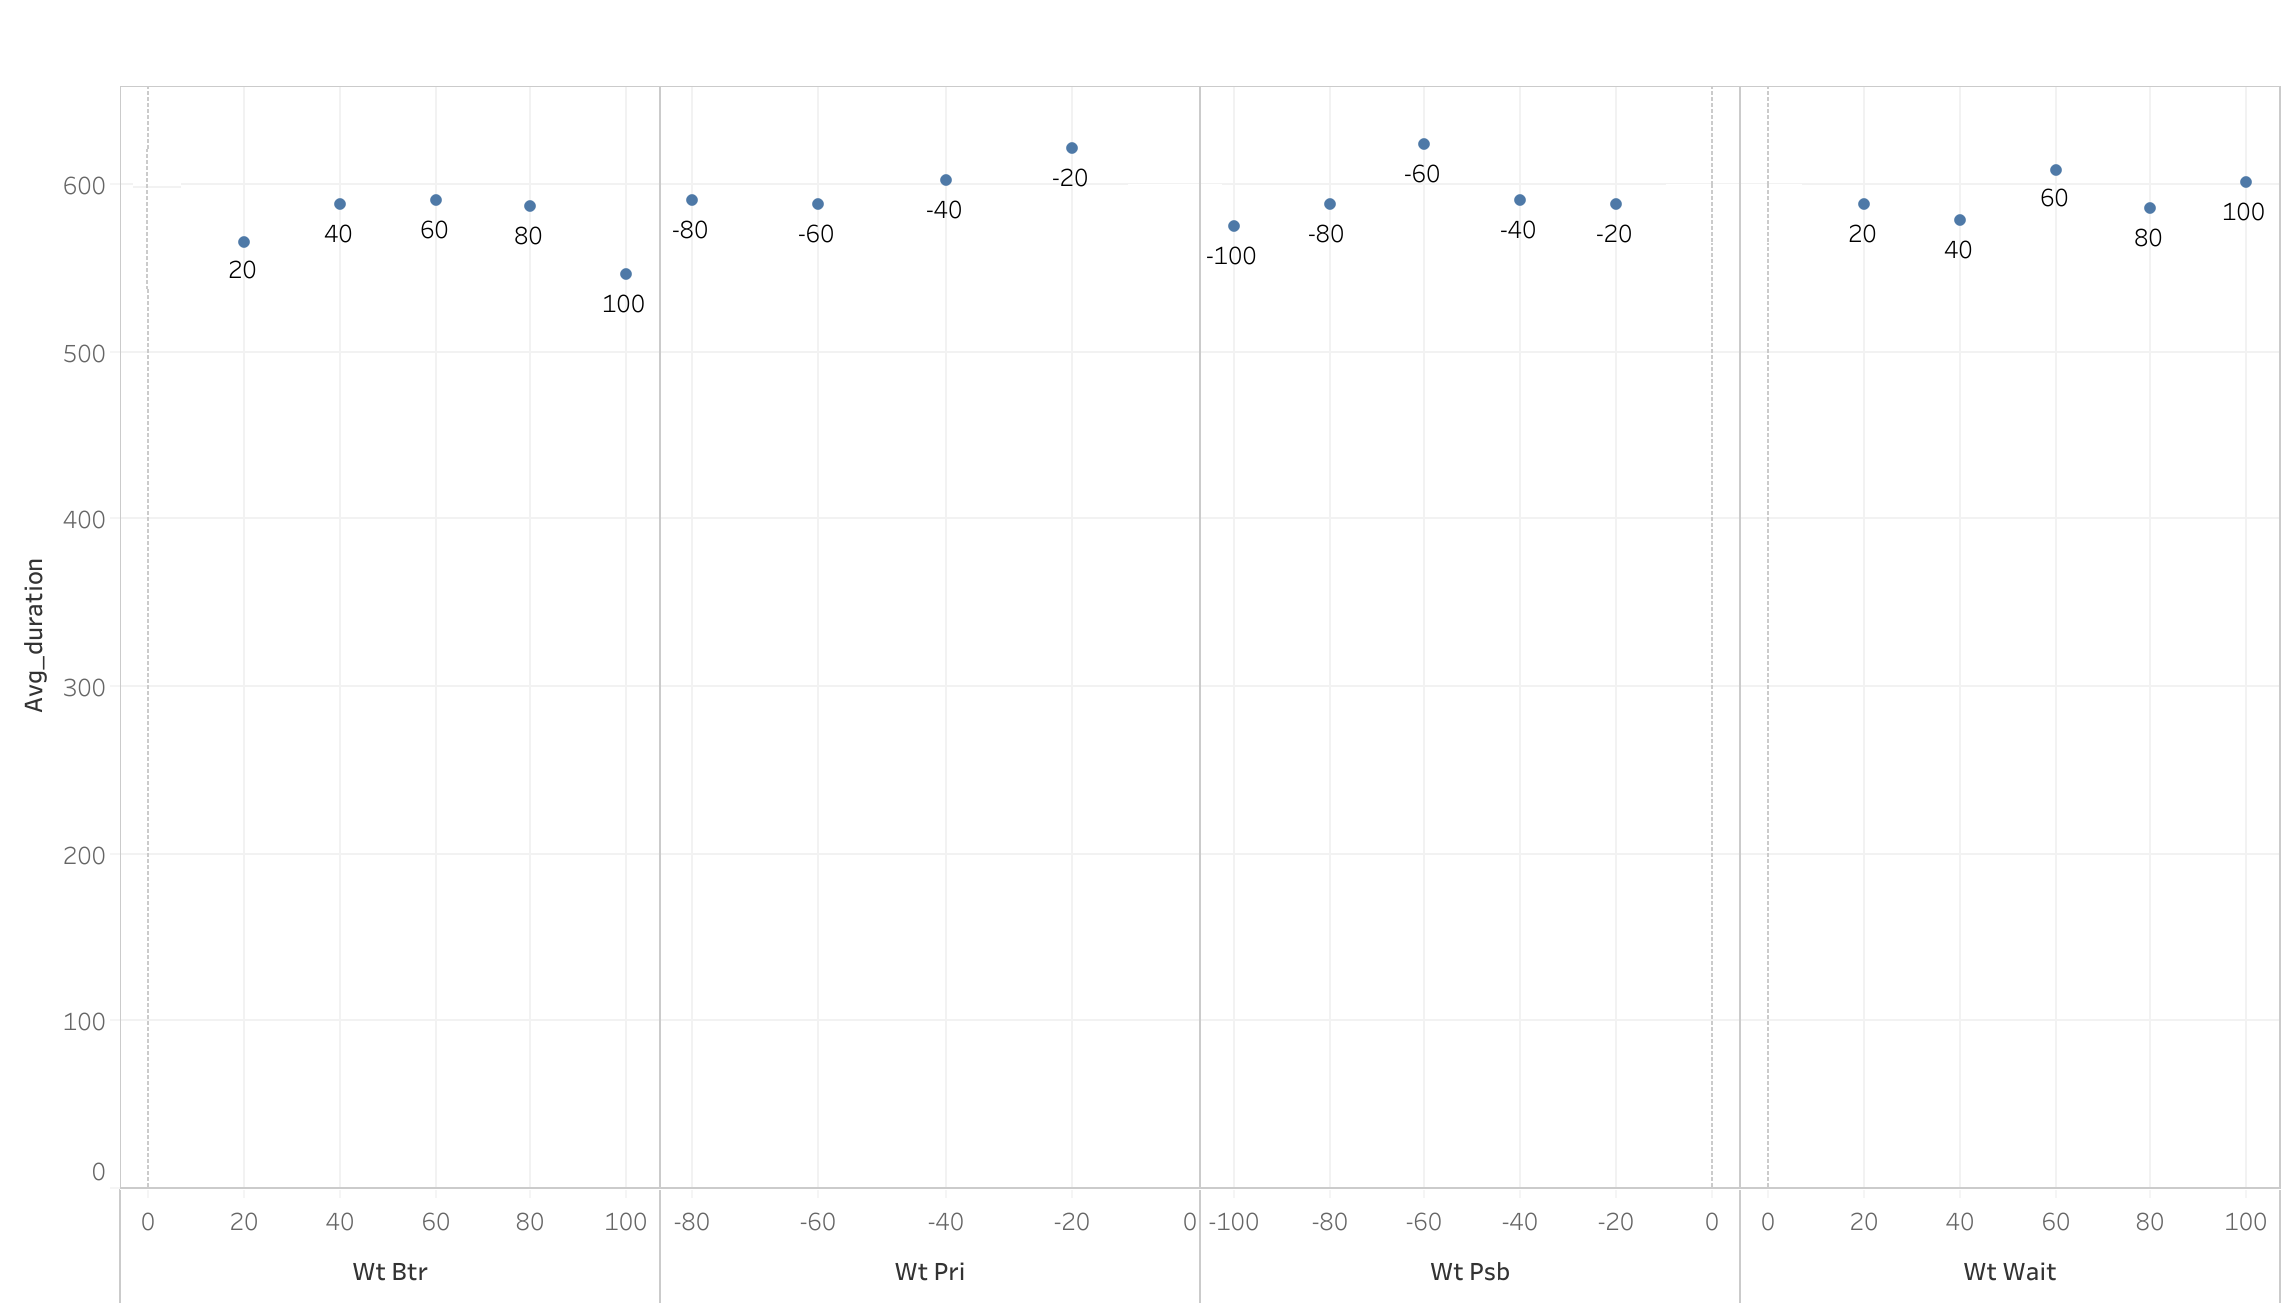
\includegraphics[width = 0.9\textwidth]{content/images/ch5/one_decision_variable.png}
    \caption{Only one desition variable changed others unchanged}
    \label{fig:only_one_desition_variable_changed}
\end{figure}

\subsection{Experiment: Find the Best Weight Combinations}
\paragraph{Experiment Introduction}
In addition to cost function, the task interval may affect experiment duration and experiment succeeded rate. Therefore, three set experiment are generated to find the best weight combinations. 
 
\paragraph{Sampling design}
Table \ref{tab:exp_task_table} shows "task table" in database. At this point, robots finished task 4-21 in experiment 1 and finished 21-39 in experiment 2. When simulation started, robots ran charging task (Task 1-3 in Table \ref{tab:exp_task_table}) and moved to corresponding charging station and started charging (Figure \ref{fig:charging_station_event}). For example, robot 1 charged at charging staion 1, robot 2 charged at charging staion 2, robot 3 charged at charging staion 3. 
    When robot fully charged, the first experiment started (Figure \ref{fig:execute_task_experiment_timeline}), and 15 ``execute tasks'' and 3 ``charging tasks'' were created (Task 4-21). Especially, in the same experiment, the task interal were the same. In Table \ref{tab:exp_task_table} the task interval was 65 seconds. In different experiment, the corresponding task had the same goal positions (Task 4 and 21, Task 4 and 22). 
    When all robot finished tasks, the experiment would be finished and robots charged at previous charging station(Task 19-21).
    These rules ensured that robot not only started at their initial positions but also processed same task set and not shuted down because of power exhaustion.


\paragraph{Analysis design}
In each experiemnt, 3 robots need to finish 15 ``execute tasks'' and 3 ``charging tasks''.
The experiment start time was when all robot finshed charging and started request task (Figure \ref{fig:execute_task_experiment_timeline}), and the experiment finish time was when the latest task is finished.
The experiment duration was an important evaluation factor, which was the time difference between experiment start time and experiment finished time.  
There end state of ``execute tasks'' were evaluated. In an experiment result table, the ``Succeeded'' column counted the tasks ended with ``Succeeded'' state, the ``Expired'' column counted the tasks ended with ``Succeeded'' state, the ``Failed'' column counted the tasks ended with ``Runing'', ``Error'', ``Canceled'', ``To rerun'' states. 
Table \ref{tab:exp_decision_variables} is an example of experiment result. 

\paragraph{Experiment Result} 
The first set of experiment uses ``execute tasks'' with 30 seconds interval. Its best weight combinations is shown in (Table \ref{tab:exp_task_30s}).
The second set of experiments used ``execute tasks'' with 45 seconds interval. Its best weight combinations is shown in (Table \ref{tab:exp_task_30s}).
The third set of experiments used ``execute tasks'' with 65 seconds interval. Its best weight combinations is shown in (Table \ref{tab:exp_task_65s}).    
\todo{Change experiment result table to graph}
\paragraph{Analysis.} 
It was concluded that the longer the task interval, the higher the task completion rate.


\begin{table}[htb]
\centering
\resizebox{\textwidth}{!}{
\begin{tabular}{|c|c|c|c|c|c|c|c|c|c|c|c|} 
\hline
$W_{\mbox{battery}}$ & $W_{\mbox{waiting time}}$ & $W_{\mbox{door open possibility}}$	&  $W_{\mbox{priority}}$ & Experiment Duration &Total Task & Succedded Task &	Expired Task & Failed Task	 \\
\hline
1 &	1 &	-1 &	-3 &	00:09:05 &	15 &	10 &	5 & 0 \\ \hline
1 &	1 &	-30 &	-1 &	00:09:05 &	15 &	10 &	5 & 0 \\ \hline
1 &	20&	-20 &	-1 &	00:09:05 &	15 &	10 &	5 & 0 \\ \hline
1 &	25&	-1 &	-1 &	00:09:05 &	15 &	10 &	5 & 0 \\ \hline
5 &	1 &	-5 &	-5 &	00:09:05 &	15 &	10 &	5 & 0 \\ \hline
\end{tabular}}
\caption{Best weight combinations with task interval 30s}
\label{tab:exp_task_30s}
\end{table}


\begin{table}[htb]
\centering
\resizebox{\textwidth}{!}{
\begin{tabular}{|c|c|c|c|c|c|c|c|c|c|c|c|} 
\hline
$W_{\mbox{battery}}$ & $W_{\mbox{waiting time}}$ & $W_{\mbox{door open possibility}}$	&  $W_{\mbox{priority}}$ & Experiment Duration &Total Task & Succedded Task &	Expired Task & Failed Task	 \\
\hline
1  & 1  & -1  & -10 & 00:11:35 & 15 & 12 & 3 & 0 \\ \hline
1  & 50 & -50 & -50 & 00:11:35 & 15 & 12 & 3 & 0 \\ \hline
25 & 20 & 0   & 0   & 00:11:35 & 15 & 12 & 3 & 0 \\ \hline
35 & 30 & 0   & 0   & 00:11:35 & 15 & 12 & 3 & 0 \\ \hline
40 & 10 & 0   & 0   & 00:11:35 & 15 & 12 & 3 & 0 \\ \hline
45 & 1  & -1  & -1  & 00:11:35 & 15 & 12 & 3 & 0 \\ \hline
50 & 50 & -50 & -1  & 00:11:35 & 15 & 12 & 3 & 0 \\ \hline
\end{tabular}}
\caption{Best weight combinations with task interval 45s}
\label{tab:exp_task_45s}
\end{table}


\begin{table}[htb]
\centering
\resizebox{\textwidth}{!}{
\begin{tabular}{|c|c|c|c|c|c|c|c|c|c|c|c|} 
\hline
$W_{\mbox{battery}}$ & $W_{\mbox{waiting time}}$ & $W_{\mbox{door open possibility}}$	&  $W_{\mbox{priority}}$ & Experiment Duration &Total Task & Succedded Task &	Expired Task & Failed Task	 \\
\hline
10.00    & 1.00     & -1.00   & 0.00    & 00:18:23 & 15    & 15  & 0  & 0     \\ \hline
1.00    & 1.00     & -1.00   & 0.00    & 00:18:23 & 15    & 15  & 0  & 0    \\ \hline
1.00    & 1.00     & -1.00   & -1.00   & 00:18:23 & 15    & 15  & 0  & 0    \\ \hline
1.00    & 5.00     & -1.00   & -1.00   & 00:18:23 & 15    & 15  & 0  & 0    \\ \hline
1.00    & 5.00     & -1.00   & -5.00   & 00:18:23 & 15    & 15  & 0  & 0    \\ \hline
1.00    & 10.00    & -10.00  & -1.00   & 00:18:23 & 15    & 15  & 0  & 0    \\ \hline
1.00    & 5.00     & -5.00   & -5.00   & 00:18:23 & 15    & 15  & 0  & 0    \\ \hline
1.00    & 5.00     & -10.00  & -5.00   & 00:18:23 & 15    & 15  & 0  & 0    \\ \hline
1.00    & 5.00     & -1.00   & -1.00   & 00:18:23 & 15    & 15  & 0  & 0    \\ \hline
1.00    & 20.00    & -1.00   & -1.00   & 00:18:23 & 15    & 15  & 0  & 0   \\ \hline
1.00    & 1.00     & -1.00   & -30.00  & 00:18:23 & 15    & 15  & 0  & 0    \\ \hline
1.00    & 1.00     & -1.00   & -35.00  & 00:18:23 & 15    & 15  & 0  & 0    \\ \hline
10.00   & 1.00     & -1.00   & -5.00   & 00:18:23 & 15    & 15  & 0  & 0    \\ \hline
10.00   & 10.00    & -1.00   & -1.00   & 00:18:23 & 15    & 15  & 0  & 0    \\ \hline
10.00   & 1.00     & -1.00   & -1.00   & 00:18:23 & 15    & 15  & 0  & 0    \\ \hline
10.00   & 1.00     & -10.00  & -1.00   & 00:18:23 & 15    & 15  & 0  & 0    \\ \hline
10.00   & 5.00     & -5.00   & -5.00   & 00:18:23 & 15    & 15  & 0  & 0    \\ \hline
10.00   & 1.00     & -10.00  & -5.00   & 00:18:23 & 15    & 15  & 0  & 0    \\ \hline
10.00   & 10.00    & -10.00  & -10.00  & 00:18:23 & 15    & 15  & 0  & 0    \\ \hline
10.00   & 1.00     & -10.00  & -1.00   & 00:18:23 & 15    & 15  & 0  & 0    \\ \hline
25.00   & 1.00     & -1.00   & -25.00  & 00:18:23 & 15    & 15  & 0  & 0    \\ \hline
30.00   & 30.00    & -1.00   & -1.00   & 00:18:23 & 15    & 15  & 0  & 0    \\ \hline
45.00   & 1.00     & -1.00   & -1.00   & 00:18:23 & 15    & 15  & 0  & 0    \\ \hline
45.00   & 1.00     & -45.00  & -1.00   & 00:18:23 & 15    & 15  & 0  & 0    \\ \hline
5.00    & 10.00    & -10.00  & -1.00   & 00:18:23 & 15    & 15  & 0  & 0    \\ \hline
5.00    & 5.00     & -1.00   & -1.00   & 00:18:23 & 15    & 15  & 0  & 0   \\ \hline
5.00    & 10.00    & -5.00   & -1.00   & 00:18:23 & 15    & 15  & 0  & 0    \\ \hline
5.00    & 5.00     & -10.00  & -1.00   & 00:18:23 & 15    & 15  & 0  & 0   \\ \hline
5.00    & 10.00    & -10.00  & -1.00   & 00:18:23 & 15    & 15  & 0  & 0    \\ \hline
5.00    & 5.00     & -1.00   & -5.00   & 00:18:23 & 15    & 15  & 0  & 0    \\ \hline
5.00    & 10.00    & -5.00   & -10.00  & 00:18:23 & 15    & 15  & 0  & 0    \\ \hline
\end{tabular}}
\caption{Best weight combinations with task interval 65s}
\label{tab:exp_task_65s}
\end{table}


\subsection{Experiment: Impact of the Number of Robots}

\paragraph{Experiment Introduction} 
In this set of experiments, how the number of robots affected task allocation was evaluated. One of the best weight combination was selected: $ W_{\mbox{battery}} = 10,W_{\mbox{waiting time}} = 1,  W_{\mbox{possibility}} = -1, W_{\mbox{priority}} = -10 $. 
    
\paragraph{Sampling design}
When simulation started, robots ran charging task and moved to corresponding charging station and started charging (Figure \ref{fig:charging_station_event}). For example, robot 1 charged at charging staion 1, robot 2 charged at charging staion 2, robot 3 charged at charging staion 3. 
When robot fully charged, the first experiment started (Figure \ref{fig:execute_task_experiment_timeline}), and 15 ``execute tasks'' and 3 ``charging tasks'' were created (Task 4-21). Especially, in the same experiment, the task interal were the same. In Table \ref{tab:task_table} the task interval was 65 seconds. In different experiment, the corresponding task had the same goal positions (Task 4 and 21, Task 4 and 22). 
When all robot finished tasks, the experiment would be finished and robots charged at previous charging station(Task 19-21).
These rules ensured that robot not only started at their initial positions but also processed same task set and not shuted down because of power exhaustion.


\paragraph{Analysis design}
As is discussed in last paragraph, in each experiemnts, robots need to finish 15 ``execute tasks'' and 3 ``charging tasks''.
The experiment start time was when all robot finshed charging and started request task (Figure \ref{fig:execute_task_experiment_timeline}), and the experiment finish time was when the latest task is finished.
The experiment duration was an important evaluation factor, which was the time difference between experiment start time and experiment finished time.  
There end state of ``execute tasks'' were evaluated. In an experiment result table, the ``Succeeded'' column counted the tasks ended with ``Succeeded'' state, the ``Expired'' column counted the tasks ended with ``Succeeded'' state, the ``Failed'' column counted the tasks ended with ``Runing'', ``Error'', ``Canceled'', ``To rerun'' states. 
Table \ref{tab:exp_decision_variables} is an example of experiment result. 

\paragraph{Result} The experiment result (Table \ref{tab:exp_robot_number}) showed that when one robot processed tasks, only 7 tasks were finished successfully; when two robots processed the same task set, 11 tasks were finished succesfully. Compared with experiment 1, experiment 2 tooks 102 seconds more but 2 more tasks were completed; when three robots processed the same task set, all 15 tasks were finished succesfully. Compared with experiment 2, the experiment duration is slightly increased but 4 more tasks were finished succesfully.

\paragraph{Analysis} It was concluded that as the number of robots increased, the task completion rate increased. However, the relationship between the number of robots and the speed of completing the task set cannot be obtained.

\begin{table}[htb]
\centering
\resizebox{\textwidth}{!}{
\begin{tabular}{|c|c|c|c|c|c|c|c|c|c|c|c|} 
\hline
Experiment & Robot number & Experiment Duration &Total Task & Succedded Task &	Expired Task & Failed Task	 \\
\hline
1 &1 &   00:16:56 & 15 & 7	& 8	& 0 \\ \hline
2 &1 &   00:16:52 & 15 & 7	& 8	& 0 \\ \hline
3 &1 &   00:17:02 & 15 & 7	& 8	& 0 \\ \hline
Average & 1 & 00:16:56 & 15	 &7	& 8 & 0\\ \hline
4 &2 &   00:19:06	& 15 & 11 & 4 & 0 \\ \hline
5 &2 &   00:18:24	& 15 & 11 & 4 & 0 \\ \hline
6 &2 &   00:18:24	& 15 & 11 & 4 & 0 \\ \hline
Average & 2 & 00:18:38 & 15	 &11	& 4	& 0 \\ \hline
7 &3 &   00:18:23	& 15 & 15 & 0 & 0 \\ \hline
8 &3 &   00:18:55	& 15 & 15 & 0 & 0 \\ \hline
9 &3 &   00:18:57	& 15 & 15 & 0 & 0 \\ \hline
Average &3 &   00:18:45	& 15 & 15 & 0 & 0 \\ \hline
\end{tabular}}
\caption{Result 4: Different number of robot processing the same task set}
\label{tab:exp_robot_number}
\end{table}


